% ! TEX root = ../pce.tex

\chapter{Curbe eliptice}
\label{ch:curbe}

\section{Generalități}

Formal, curbele eliptice sînt varietăți proiective de dimensiune 1 și gen 1,
dar ele pot fi definite și intuitiv, la nivel elementar, folosind forma
dată de așa-numita \emph{ecuație Weierstrass}.

Fără a intra în detalii generale privitoare la funcțiile Weierstrass, este
suficient să definim o \emph{curbă eliptică} printr-o ecuație de forma:
\[
  y^2 = x^3 + ax + b,
\]
care este \emph{nesingulară}, adică nu conține \qq{colțuri} (eng.\ \emph{cusps})
și autointersecții. În funcție de corpul peste care este definită curba
eliptică, coeficienții $ a, b $ sînt elemente ale corpului respectiv.

Clasificarea curbelor eliptice se face folosind \emph{discriminantul} curbei,
care se definește prin:
\[
  \Delta = -16(4a^3 + 27b^2),
\]
care trebuie să fie nenul ca să avem o curbă nesingulară.

Aplicațiile în geometrie algebrică și criptografie sînt facilitate de posibilitatea
definirii unei structuri de grup pe mulțimea punctelor de pe o curbă eliptică.
Această structură de grup este bine precizată riguros, folosind \emph{divizori}
(cf., de exemplu, \cite{sil09}, III.\S2), dar pentru scopurile lucrării prezente
va fi suficient să descriem operația de grup intuitiv.

Astfel, fie $ P $ și $ Q $ două puncte de pe curbă. Putem descrie punctul $ P + Q $
astfel: se trasează dreapta care conține cele două puncte și al treilea punct
de intersecție al acestei drepte cu curba se definește ca fiind opusul rezultatului.

Formal, avem:
\begin{definition}\label{def:adunare-pc}
  Fie $ E $ o curbă eliptică și fie $ P, Q $ două puncte pe $ E $.

  Fie $ L $ dreapta prin $ P $ și $ Q $ (dacă $ P = Q $, atunci $ L $ va
  fi tangenta în $ P $). Fie $ R $ un al treilea punct de intersecție al
  lui $ L $ cu $ E $.

  Fie $ L' $ dreapta care unește $ R $ și $ O = [0, 1, 0] $, punctul de la
  infinit.

  Atunci $ L' $ intersectează $ E $ în $ R, O $ și un al treilea punct,
  care se notează $ P + Q $.
\end{definition}

Operația este ilustrată în figura \ref{fig:pc-adunare}
\begin{figure}[!htbp]
  \centering
  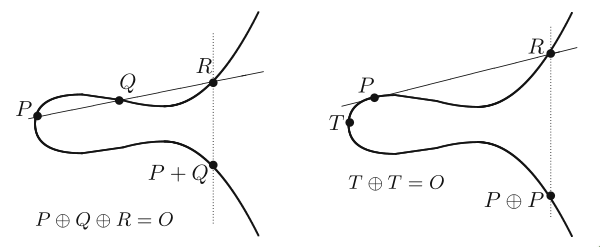
\includegraphics[scale=0.5]{fig/adunare-el.png}
  \caption{\textit{Adunarea punctelor pe o curbă eliptică, \cite{sil09}, p.\ 51}}
  \label{fig:pc-adunare}
\end{figure}

Cu această operație $ (E, +) $ formează un grup abelian, cu elementul neutru
$ O = [0, 1, 0] $.

\begin{example}\label{exm:adunare-pc}
  Fie curba eliptică $ E $, definită peste $ \QQ $ prin ecuația Weierstrass:
  \[
    E : y^2 = x^3 + 17.
  \]
  Calcule simple găsesc cîteva puncte cu coordonate întregi:
  \[
    P_1 = (-2, 3), \quad P_2 = (-1, 4), \quad P_3 = (2, 5), \quad P_4 = (4, 9), %
    \quad P_5 = (8, 23).
  \]
  Folosind operația de grup, putem verifica relațiile:
  \[
    P_5 = -2 \cdot P_1, \quad P_4 = P_1 - P_3.
  \]

  Mai general, de fapt, se poate arăta că orice punct rațional $ P \in E(\QQ) $
  poate fi scris sub forma:
  \[
    P = mP_1 + nP_3, \quad m, n \in \ZZ,
  \]
  de unde rezultă că $ E(\QQ) = \ZZ \times \ZZ $.
\end{example}

%%%%%%%%%%%%%%%%%%%%%%%%%%%%%%%%%%%%%%%%%%%%%%%%%%%%%%%%%%%%%%%%%%%%%%

\section{Aplicația Frobenius}

Lucrăm în cazul particular cînd curba $ E $ este definită peste un corp finit
$ \FF_q $ (caz dezvoltat și în secțiunile următoare). Așadar, considerăm
$ q $ o putere a unui prim $ p $, iar $ \FF_q $ va fi corpul cu $ q $
elemente.

Se definește \emph{aplicația Frobenius} prin:
\[
  \phi : E \to E, \quad \phi(x, y) = (x^q, y^q).
\]

Mai general, dacă $ K $ este un corp care-l extinde pe $ \FF_q $,
se poate defini morfismul Frobenius $ F $ în general prin
$ \alpha \mapsto \alpha^q $.

Cîteva proprietăți elementare, preluate fără demonstrație din \cite{soe}:
\begin{proposition}\label{pr:propr-frob}
  Aplicația $ F : K \to K $ de mai sus satisface proprietățile:
  \begin{enumerate}[(a)]
  \item $ F(xy) = F(x) F(y), \forall x, y \in K $;
  \item $ F(x + y) = F(x) + F(y), \forall x, y \in K $;
  \item $ \FF_q = \{ \alpha \in K \mid F(\alpha) = \alpha \} $;
  \item Dacă $ K = \FF_q(t) $ este corpul de funcții raționale
    peste $ \FF_q $, într-o nedeterminată $ t $, atunci pentru o funcție
    rațională $ \gamma \in \FF_q(t) $ are loc $ F(\gamma(t)) = \gamma(t^q) $.
  \end{enumerate}
\end{proposition}

Demonstrațiile sînt manipulări algebrice simple ale proprietăților corpurilor
finite, precum și ale caracteristicii $ q $, în mod esențial.

De asemenea, aplicația Frobenius este bijectivă.

%%% Local Variables:
%%% mode: latex
%%% TeX-master: "../pce"
%%% End:
